\afterpage{\clearpage}
%\subsection{Pause Analysis}

\section{Symbol Models}
For an explanation on the Symbol Model notation please refer to the glossary.

\subsubsection{Symbol Model Approach 1} 
This symbol model was created to test the effectiveness of SMA1. 
From the data in the pause analysis section, 50\% of the pauses were 100ms and 200ms.
From this the maximum entropy can be achieved for the ABC files on average using a model of [3], therefore
Symbol Model [3] (SM[3]) was used. 
%\begin{itemize}
%\item $A < 300ms$
%\item $B > 300ms$
%\end{itemize}

\subsubsection{Investigating Bin Width and Outlier Visualisation}
These models were created to investigate how bin width change simple binary models and look at the effect outlier symbols have on the entropy profile. This was used to investigate initial classification potential by analysing how the entropy profile behaves where the margin between the symbols occurrences was increased incrementally to produce outliers. 
The symbol models used were: \\
Symbol Model [10] (SM[10]) \\
Symbol Model [20] (SM[20]) 
%Symbol Model [35] (SM[35])
%Showing obvious anomalies at two points in the audio recording. Given a rare enough event, this shows it can be picked up, recorded and displayed. In this case separating the file into bins of above or below 20 likely has no meaning. But this is a good test. \\
%\begin{itemize}
%\item $A < 1000ms$
%\item $B > 1000ms$
%\end{itemize}
%
%\subsubsection{Symbol Model [20] (SM[20])}
%This model was created to investigate other simple models.
%Using an investigative approach to explore how the entropy profile changes, this symbol model was defined as:
%\begin{itemize}
%\item $A < 2000ms$
%\item $B > 2000ms$
%\end{itemize}

%But this model doesn't include the 5\% variance? 236 is 5\% of 4725. 
%Although this approach may seem too simple, its purpose is to give initial insight without diving too much into any one direction. Further tests will include creating the symbol set be more robust to variance by including a 5\% margin of variance to be accounted for. More sophisticated averaging techniques. Machine Learning. ...
%From this symbol model the conversations above would be classified correctly?

\subsubsection{Symbol Model Approach 2}
This model was created to test the effectiveness of SMA2. 
Figure 5.23 was used from Symbolisation Approach 2 to define this symbol model as as: \\
Symbol Model [3,6,10,15] (SM[3,6,10,15])}

%\subsubsection{Symbol Model [3,6,10,15] (SM[3,6,10,15])}

%\begin{itemize}
%\item $A < 300ms$
%\item $B < 600ms$
%\item $C < 1000ms$
%\item $D < 1500ms$
%\item $E > 1500ms$
%\end{itemize}


%\begin{figure}[h]
%\begin{center}
%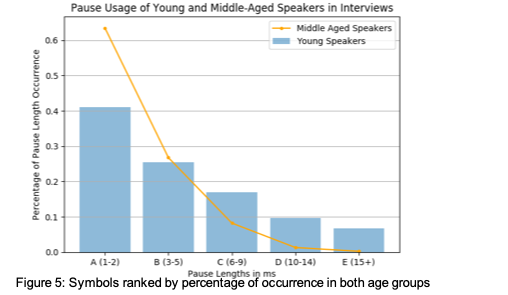
\includegraphics{src/main-matter/results/experiment-age/symbol-model/SM2}
%\caption{SM2 ranked probability showing the margin difference for both groups}
%\label{default}
%\end{center}
%\end{figure}

%\subsubsection{Investigating Symbol Model Size Increase}
%These models were created to investigate adding complexity to a model through increasing symbol model size.
%Using an investigative approach to explore how the entropy profile changes, these symbol models were defined as:\\
%Symbol Model [2,3,4,5] (SM[2,3,4,5]) \\
%Symbol Model [2,3,4,5,6] (SM[2,3,4,5,6]) \\
%Symbol Model [2,3,4,5,6,7] (SM[2,3,4,5,6,7]) \\
%Symbol Model [2,3,4,5,6,7,8] (SM[2,3,4,5,6,7,8]) \\
%Symbol Model [2,3,4,5,6,7,8,9] (SM[2,3,4,5,6,7,8,9]) \\



%\subsubsection{Symbol Model [2,3,4,5,6,7,8,9,10] (SM[2,3,4,5,6,7,8,9,10])}
%This model was created to investigate adding complexity to a model.
%Using an investigative approach to explore how the entropy profile changes, this symbol model was defined as:

%\begin{itemize}
%\item $A < 200ms$
%\item $B < 300ms$
%\item $C < 400ms$
%\item $D < 500ms$
%\item $E < 600ms$
%\item $F < 700ms$
%\item $G < 800ms$
%\item $H < 900ms$
%\item $I < 1000ms$
%\item $J > 1000ms$
%\end{itemize}

%Using this average calculated above, the ranked probability will become A, B, C, J, D, E, F, G, H, I. 





%Another table showing the variance between symbol counts. Aim: try equalising values to minimise the drop or gate between symbols
%to utilise as many pauses as possible. Constraint: the grain is at the finest it can be, so no split can be done to further reduce symbols,
%but groups can be joined. Warning though, if groups are joined then the new variance of this group could overlap with another symbol 
%meaning audio files cant be distinguished purely through symbol ranking. Question, will symbol ranking necessarily make the anomaly 
%plot work better or best? Can I use the ranked probability to get the zml? What I would really want is histograms lined up side by side 
%that can be easily broken into groups, but the finest detail I can get is 1ms. Need to work as best as I can with 1ms? 

%5\% of the total pauses






